\documentclass{beamer}

\usetheme{Warsaw}
%\usetheme{Antibes}
%\usetheme{JuanLesPins}
%\usetheme{Goettingen}

%\usecolortheme{seahorse}
%\usecolortheme{dolphin}
\usecolortheme{rose}
% http://deic.uab.es/~iblanes/beamer_gallery/index_by_color.html
%\usecolortheme{beaver}

%\useoutertheme[]{sidebar}

\setbeamercovered{transparent}

\usepackage[slovak]{babel}
\usepackage[T1]{fontenc}
\usepackage[utf8]{inputenc}
\usepackage{url}

\usepackage{listings}

\lstset{language=C++,basicstyle=\fontsize{8}{9.6}\selectfont,showstringspaces=false,columns=fullflexible,identifierstyle=\ttfamily,keywordstyle=\bfseries,showstringspaces=false,columns=fullflexible}
%\lstset{language=C,basicstyle=\fontsize{10.5}{12.6}\selectfont,identifierstyle=\ttfamily,keywordstyle=\bfseries,showstringspaces=false,columns=fixed}

\def\BibTeX{\textsc{Bib}\kern-.08em\TeX} 

\newcommand{\footcite}[1]{\footnote{\tiny #1}}
\newcommand{\umlet}{.5}
\newcommand{\emp}[1]{\textit{\alert{#1}}}
\newcommand{\kw}[1]{\mbox{\textbf{#1}}}
\newcommand{\id}[1]{\texttt{#1}}
\newcommand{\stl}{\guillemotleft}
\newcommand{\str}{\guillemotright}

\newcommand{\lsti}{\lstinline[basicstyle=\fontsize{10.5}{12.1}\selectfont]}

\newcommand{\ssection}[1]{
	\section{#1}
	\begin{frame}[fragile=singleslide]\frametitle{}
	\Huge #1
	\end{frame}
}

\newcommand{\ssectionn}[1]{
	\section*{#1}
	\begin{frame}[fragile=singleslide]\frametitle{}
	\Huge #1
	\end{frame}
}

\newenvironment{program}{\begin{beamercolorbox}[rounded=true,shadow=true]{block body}\vspace{-4mm}}{\vspace{-2mm}\end{beamercolorbox}}

\setbeamercolor{fvystup}{fg=white,bg=black}
\newenvironment{vystup}{\begin{beamercolorbox}[rounded=true,shadow=true]{fvystup}}{\end{beamercolorbox}}

\newenvironment{poznamka}{\begin{beamercolorbox}[rounded=true,shadow=false]{block body}}{\end{beamercolorbox}}

\setbeamertemplate{footline}[page number]
{
%\insertpagenumber
%\begin{beamercolorbox}{section in head/foot}
%\vskip2pt\insertnavigation{\paperwidth}\vskip2pt
%\end{beamercolorbox}%
}



\author{Samuel Petrík}

\institute{
	Fakulta informatiky a informačných technológií\\
	Slovenská technická univerzita v Bratislave}

\title{Využitie virtuálnej reality vo vzdelávaní v
medicíne
}

\date{\footnotesize 24. november 2022}




\begin{document}

\begin{frame}[fragile=singleslide]
\titlepage
\end{frame}


\begin{frame}[fragile=singleslide]\frametitle{Obsah}
\begin{itemize}
\item Virtuálna realita
\item Využitie VR vo výuke medicíny
\item Štúdie o využití VR v Bulharsku
\item Dištančné vyučovanie s VR
\end{itemize}
\end{frame}


\begin{frame}[fragile=singleslide]\frametitle{Virtuálna realita}
\begin{itemize}
\item odomyká nové možnosti
\item nové zručnosti a skúsenosti
\item interaktívne prostredie
\end{itemize}
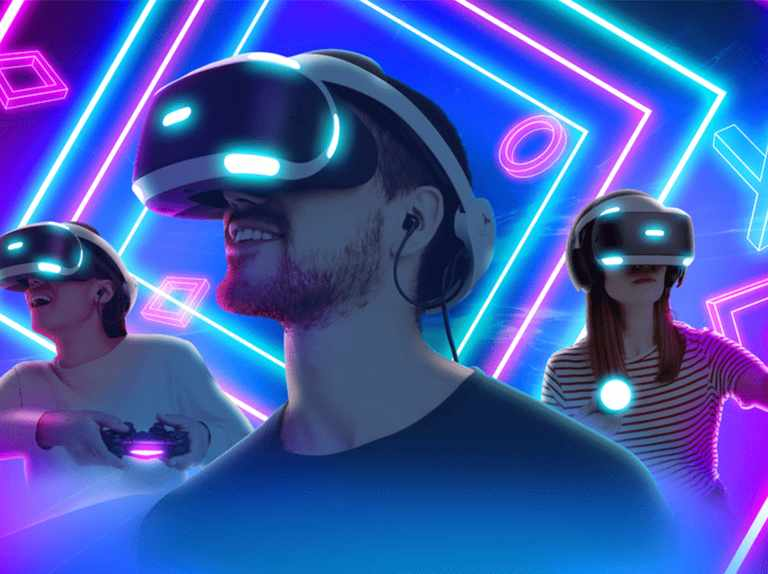
\includegraphics[scale=.2]{VR.jpg}
\end{frame}

\begin{frame}[fragile=singleslide]\frametitle{Využitie VR vo výuke medicíny}
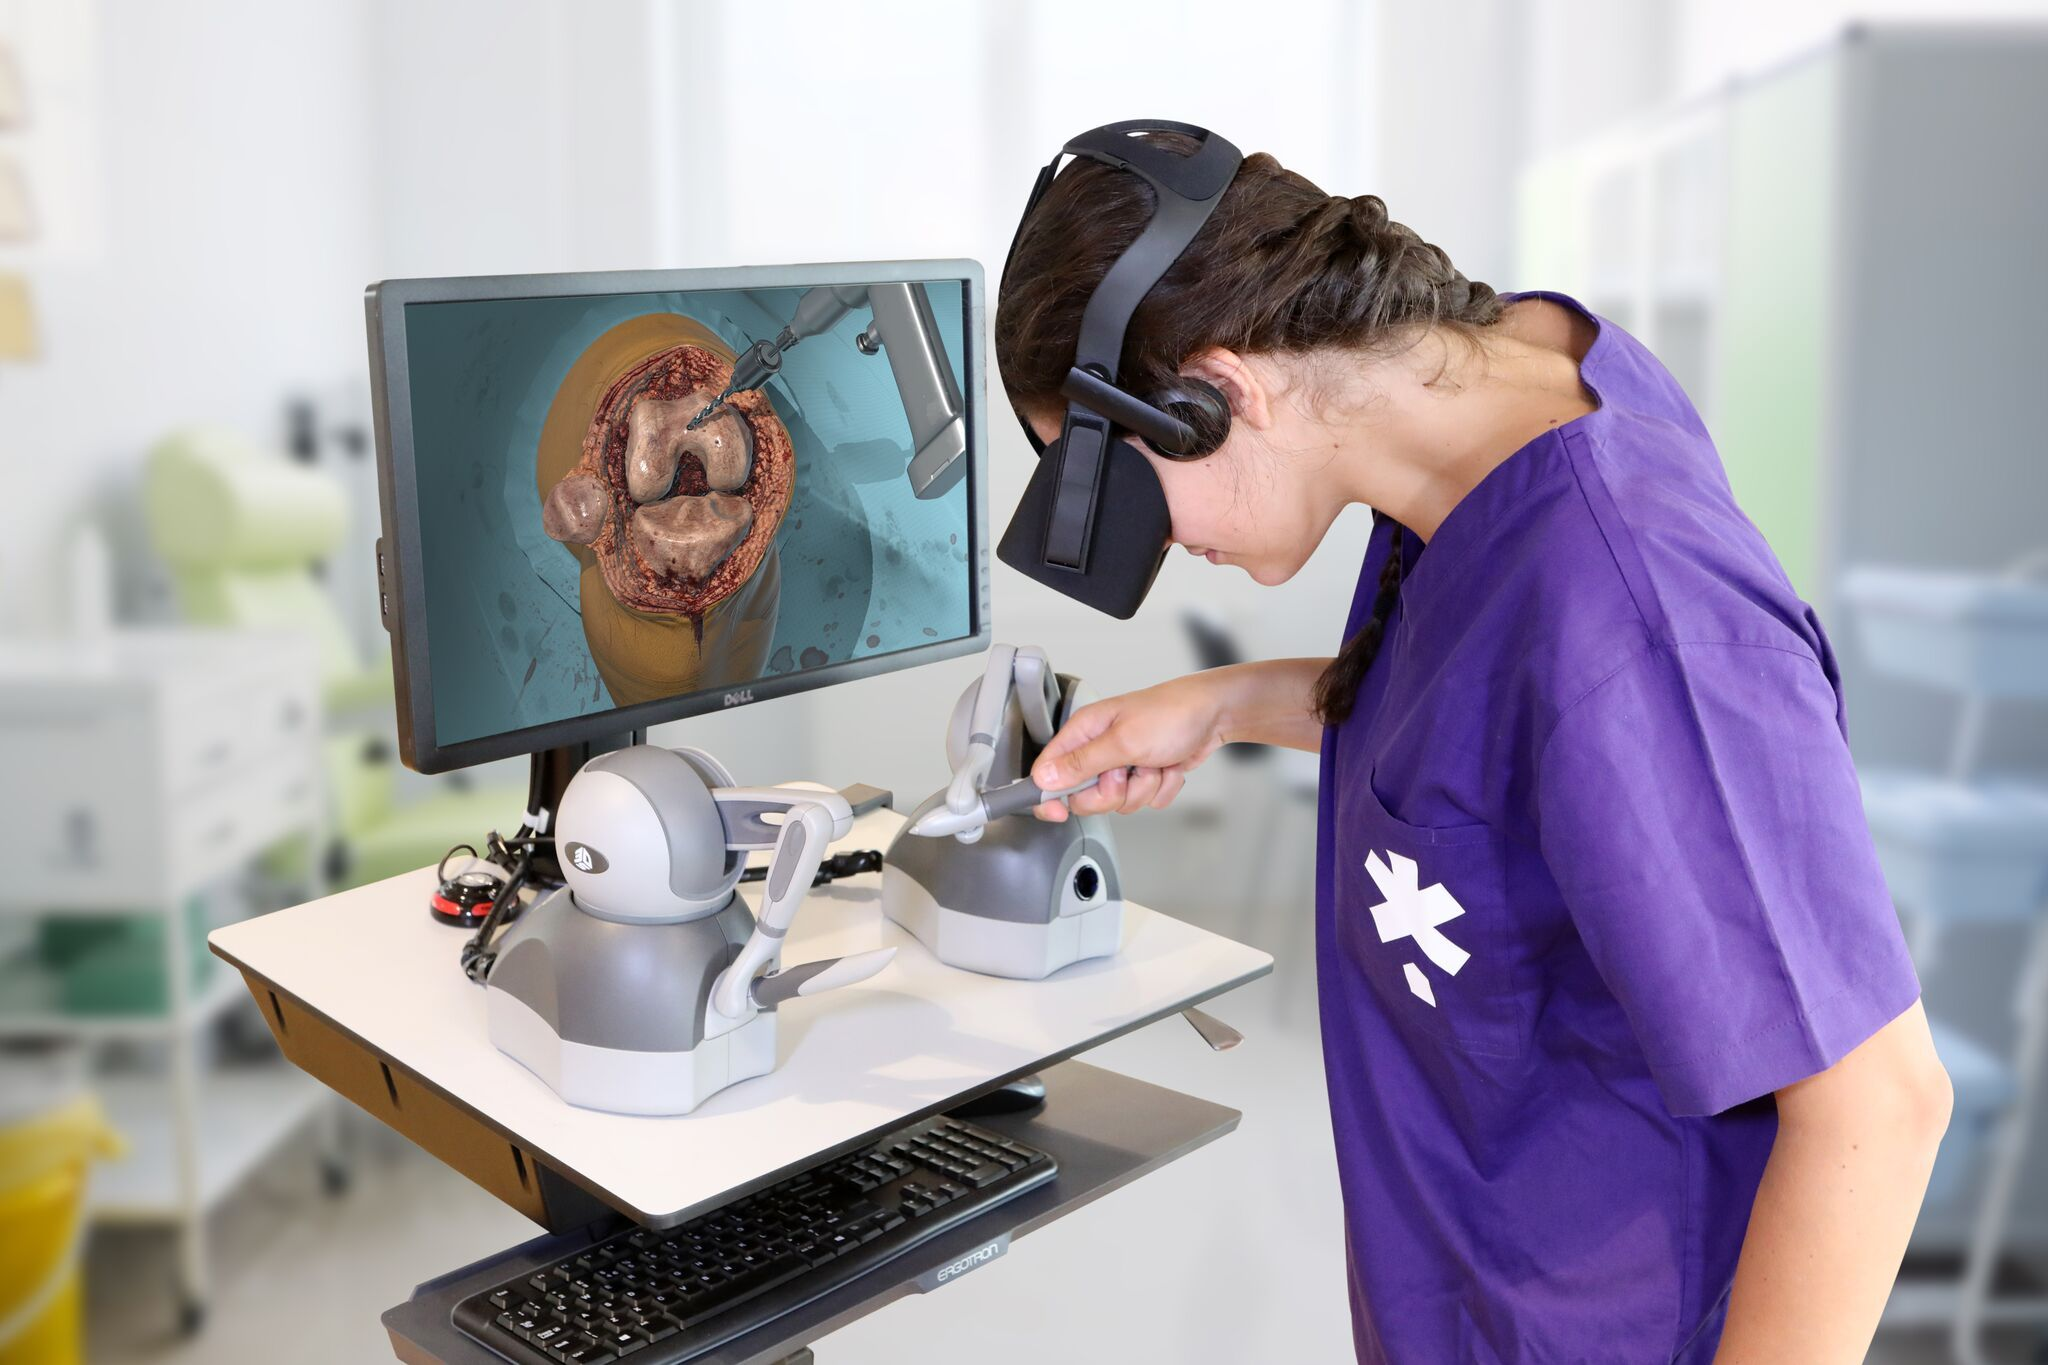
\includegraphics[scale=.1]{VRM.jpeg}
\begin{itemize}
\item efektívnejšie učenie 
\item nadobudnutie sebavedomia
\item Virtual 3D Atlas of Human Body
\end{itemize}
\cite{Clanok2}
\end{frame}


\begin{frame}[fragile=singleslide]\frametitle{Štúdie o využití VR v Bulharsku}
\begin{itemize}
\item časť prezentovanej štúdie
\end{itemize}
\cite{Clanok1}
\includegraphics[scale=.7]{tabuľka.pdf}
\cite{Clanok1}
\end{frame}


\begin{frame}[fragile=singleslide]\frametitle{Dištančné vyučovanie s VR}
\begin{itemize}
\item pandémia spôsobila zatváranie škôl
\item vyýuka mala zhoršenú kvalitu
\item nové možnosti vďaka VR
\end{itemize}

\includegraphics[scale=1]{DV.jpg}
\end{frame}


\begin{frame}[fragile=singleslide]\frametitle{Ďakujem za pozornosť}
Zdroje :
\bibliography{literatura}
\bibliographystyle{plain}
\begin{itemize}
\item https://www.worldbank.org/en/topic/edutech/brief/edtech-toolkit-for-remote-learning
\item https://onix-systems.com/blog/implementing-virtual-reality-in-medicine-and-medical-training
\item https://www.radiotimes.com/technology/gaming/ps5-vr-release-date-price-upgrade/
\end{itemize}
\end{frame}


\end{document}
